\chapter{Introduction}
    %\addcontentsline{toc}{chapter}{\protect\numberline{}Introduction}
    
     % Might be useful: http://www.emerson.emory.edu/services/latex/latex_162.html

\section{General context}

%Since its early days, humankind has always felt the desire to fly. 

%It was not until the World War I, when planes took a fundamental role in the last stages of the 

%In World War I, airplanes played a fundamental role 


In the 20th century, the field of aeronautics has experimented a hectic growth since World War I (1914 - 1919), when airplanes played a fundamental role in the aerial battles. The advances in military aviation led to the apparition of the first airlines and the birth of commercial aviation after the war. It was not, however, until World War II (1939 - 1945) that the biggest progresses were made: technological improvements resulted in larger, more efficient aircrafts that were used for surveillance, in air battles or for bombing purposes. After this period, airplanes used during the war were recycled with civil purposes to transport cargo and passengers. This supposed the beginning of a new era for commercial aviation that has not stopped to grow until nowadays, where air transportation is an essential activity in today's society.

The increasing relevance of commercial aviation has been possible due to advances in aeronautical technologies, from structures and control systems to propulsion systems. In the case of the latter, the birth of the jet engine in the 1930s supposed a milestone that marked the transition from propelled airplanes working with internal combustion engines to faster ones powered by gas turbines. Improvements in propulsion technologies have led to bigger, more efficient engines which can produce more power in order to drive bigger airplanes faster during longer times, hence covering longer distances. 

%However, despite today's propulsion technologies being more efficient than those from its origins, they are not extent of pollutant emissions. The increasing demand of commercial transportation in the last years, as well as the increasing general concern for the effects of greenhouse gases on climate change, has made the aeronautical engine manufactures to place emissions' reduction as a major constraint for engine design. In this respect, pollutant species such as CO, CO$_2$ and NO$_\mathrm{x}$, generated during the combustion process, are meant to be reduced. 

However, despite today's propulsion technologies being more efficient than those from its origins, they are not extent of producing emissions. Species generated during the combustion process in gas turbines include CO$_2$, a greenhouse gas contributing to global warming, and CO and NO$_\mathrm{x}$, considered as pollutant emissions. In this respect, the increasing demand of commercial transportation and a rising general concern about the effects of climate change, have placed the need of reducing emissions, as well as noise, as a major constraint for the development of aviation in the decades to come. The Advisory Council of Aeronautic Research in Europe (ACARE) has settled the goal to reduce the emissions per passenger/kilometre of CO$_2$ by 75 $\%$ and of NO$_\mathrm{x}$ by 90 $\%$ for the year 2050 with respect to the levels of 2000 \citepColor[acare_strategic_2017].

Emissions of NO$_\mathrm{x}$ are a big concern due to their harmful effect in health and environment (e.g. it is one of the main species producing acid rain). The evolution of aeronautical engines in the last decades have led to higher combustion temperatures and larger Overall Pressure Ratios (OPR), which help to reduce fuel consumption but increase the production of NO$_\mathrm{x}$. Engine manufacturers have worked on mitigating this increasing trend, as shown by the evolution of NO$_x$ emissions with OPR for several generations of engines in Figure \ref{fig:NOX_emissions_with_OPR}. It is shown how certified engines have succeeded in reducing emissions below the ICAO-CAEP regulatory limits. Nevertheless, the NO$_\mathrm{x}$ are still expected to grow due to the expanding aerial traffic demand. Figure \ref{fig:NOX_forecasts} displays the forecasts for several traffic scenarios, where it is shown the potential effect of technology advances in the emissions at 2040 (lower bounds) with respect to the case where current technologies (of year 2017) would be used (upper bounds). Therefore, in order to maintain the emissions below a certain level and hence accomplish the ACARE goals, substantial efforts need to be done. One way of achieving this is by controlling and improving the combustion process, since it is known that NO$_\mathrm{x}$ are produced at high temperatures. For this purpose, the aeronautical community is working towards new combustion chambers and injection processes aiming at creating \textbf{lean combustion}.

\begin{figure}[h!]
	\centering
	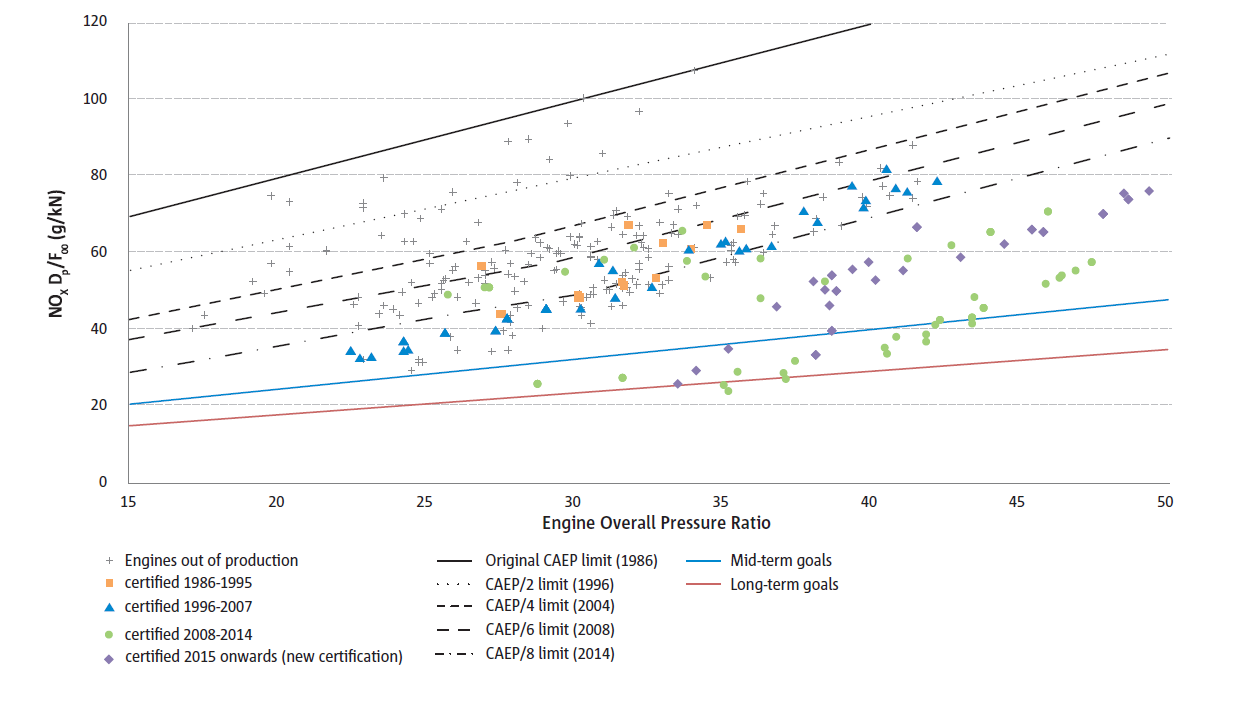
\includegraphics[scale=0.6]{./part0_intro/NOx_emissions_with_OPR}
	\caption{Evolution of NO$_x$ emissions with several generations of aircraft engines. Source: \citepColor[easa_european_2019]}
	\label{fig:NOX_emissions_with_OPR}
\end{figure}

\begin{figure}[h!]
	\centering
	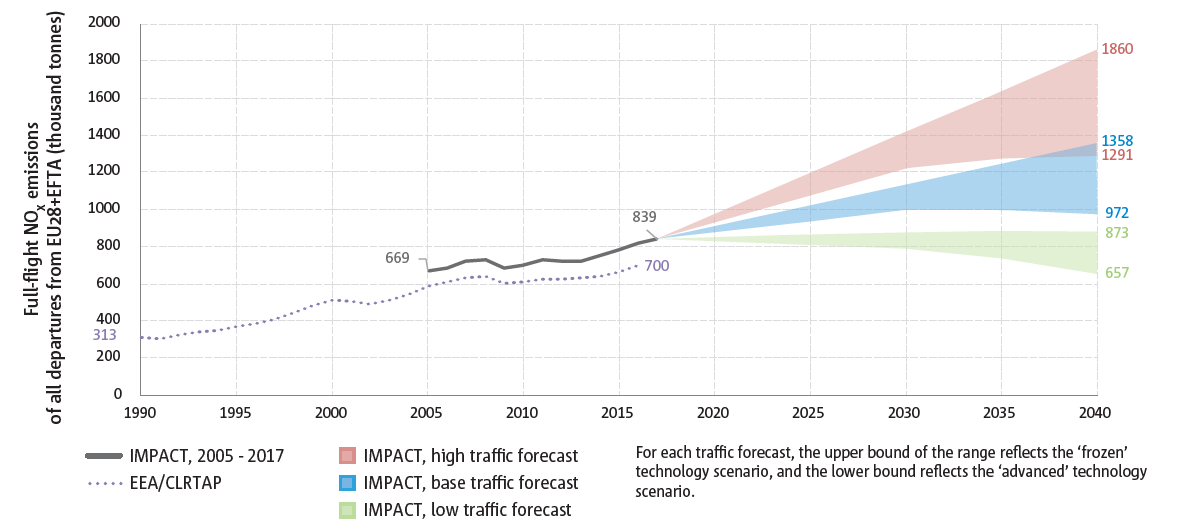
\includegraphics[scale=0.6]{./part0_intro/NOx_emissions_forecast_report2019}
	\caption{NO$_x$ emission forecasts from 2017 to 2040. Source: \citepColor[easa_european_2019]}
	\label{fig:NOX_forecasts}
\end{figure}


\section{Lean combustion in aeronautical gas turbines}

%Conventional combustors used to introduce only a small portion of air ($\sim 30 \%$ ) with the liquid injection system, and the rest was introduced through secondary holes located downstream (see Figure \ref{fig:combustor_conventional}). As a consequence, com

%\begin{figure}[h!]
%	\centering
%	\includegraphics[scale=0.6]{./part0_intro/combustor_conventional}
%	\caption{Conventional combustor. Source: \citeColor[lefebvre_gas_2010].}
%	\label{fig:combustor_conventional}
%\end{figure}

With the objective of reducing NO$_\mathrm{x}$ emissions in aeronautical engines, the community has worked towards the implementation of concepts aiming at producing lean combustion. The motivation for developing lean systems is shown in Figure \ref{fig:NOX_motivation_and_RQL} left: at lean regimes (i.e. with an excess of air), the flame temperature is lower and, consequently, NO$_\mathrm{x}$ formation is reduced. At the same time, emissions of CO, hydrocarbons (HC) and soot are also diminished at this regime (provided that the air excess is not too high, or the emissions will start to grow again). On the other hand, operating at lean regimes will make the system more prone to thermoacoustic instabilities and will place it closer to the the limit of lean blow-out (LBO), hindering ignition and relight capabilities. 

One of the first concepts aiming at reducing emissions is the \textbf{Rich-Burn, Quick-Quench, Lean-Burn} (\textbf{RQL})  \citepColor[novick_low_1981]. RQL systems split the combustion process in three stages. Firstly combustion begins in a fuel-rich primary zone close to the injector, where the NO$_\mathrm{x}$ rate is low (see Figure \ref{fig:NOX_motivation_and_RQL} left). Then, a quick mixing of the unburnt fuel takes place with fresh air to finally burn in lean conditions. This procedure allows to decrease NO$_\mathrm{x}$ emissions as depicted by the low-NO$_\mathrm{x}$ route depicted in Figure \ref{fig:NOX_motivation_and_RQL}. However, a fine and complete fuel atomization is needed so that a fast mixing takes place; otherwise, unburnt fuel could produce extra smoke and soot in the rich-burn region \citepColor[el-asrag_simulation_2007]. This hinders the proper operation of RQL chambers in regimes where fuel can hardly be atomized, such as during altitude relight.

\begin{figure}[h!]
	\centering
	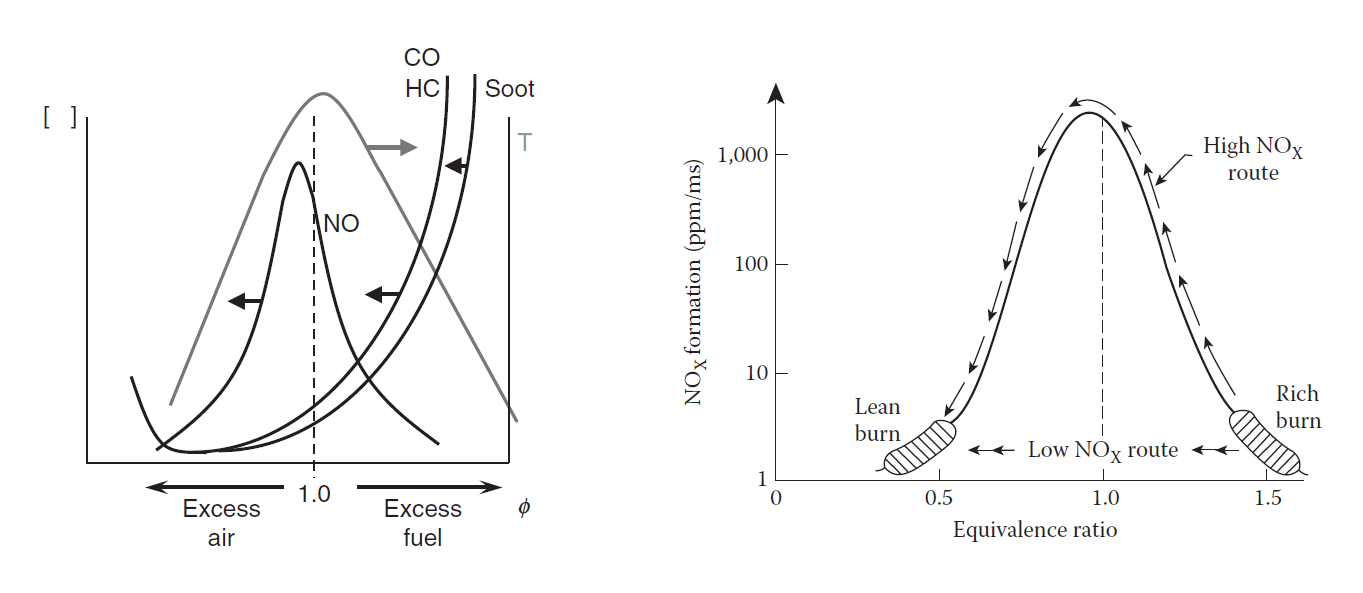
\includegraphics[scale=0.65]{./part0_intro/NOX_motivation_and_RQL}
	\caption{\textsl{Left}: Temperature and species concentration variation with stoichiometric ratio in combustion chambers. Source: \citeColor[dunn-rankin_lean_2008]. \textsl{Right}: NOx formation in Rich-Burn, Quick-Quench, Lean-Burn (RQL) concepts. Source: \citeColor[lefebvre_gas_2010].}
	\label{fig:NOX_motivation_and_RQL}
\end{figure}

The need of reducing NO$_\mathrm{x}$ emissions to the levels settled by authorities led to the development of lean combustion strategies, usually referred as low-NO$_\mathrm{x}$ \citepColor[tacina_low_1990]. In order to foster lean combustion, low-NO$_\mathrm{x}$ concepts introduce an excess of air at the vicinity of the injector: around $70 ~\%$ of air is introduced in the combustion chamber at this location (primary zone), while the rest is used further downstream for effusion cooling. Compared to conventional combustors, where around $30 ~\%$ of air is injected in the primary zone and the rest is introduced further downstream through dilution holes, this allows to reduce the length of the combustion chamber and hence the residence time of combustion, directly linked to NO$_\mathrm{x}$ formation \citepColor[lefebvre_gas_2010]. Furthermore, operating directly at lean regimes will also reduce the formation of soot and CO emissions, which is the main disadvantage of RQL. One of the first lean combustion concepts is the \textbf{Lean Direct Injection} (\textbf{LDI}) technology \citepColor[tacina_low_1990], where fuel is directly introduced into the reaction zone without previous premixing. Lower peak temperatures and residence times are obtained, hence reducing pollutant formation. Contrarily, LDI concepts can produce a non-uniform combustion if mixing is not complete. In this respect, the \textbf{Lean Premixed Prevaporized} (\textbf{LPP}) technology appeared to palliate this issue \citepColor[bittlinger_high_1999]: a premixing length is added before the reaction zone, so that complete evaporation of fuel and mixing can take place before triggering combustion. LPP concepts need, however, a longer combustion chamber to account for the dilution zone, and are more prone to suffer autoignition, flashback and thermoacoustic instabilities.

A good trade-off between both LDI and LPP is obtained with \textbf{Multi-Staged Fuel Injection} (MSFI) \citepColor[pehanhoat_low_2006]. Fuel is introduced in the combustion chamber through two main stages: a \textbf{pilot stage} for flame stabilization purposes, and a \textbf{take-off stage} (also called multipoint ) where the most of premixing takes place (see Figure \ref{fig:foust_TAPS} left). The combination of both injection systems creates a flame that burns in lean conditions and reduces combustion instabilities compared to other low-NO$_\mathrm{x}$ concepts \citepColor[barbosa_time_2009]. The percentage of fuel introduced through each stage can be controlled in order to optimize the combustion performance depending on the flight phase: this procedure is called staging. Considerable reductions in emissions can be obtained with MSFI in conditions where most of NO$_\mathrm{x}$ is produced, such as climb and cruise. Figure \ref{fig:foust_TAPS} right shows the improvements in pollution of a multi-staged fuel injector named Twin Annular Premixing Swirler (TAPS) \citepColor[foust_development_2012] compared to a RQL combustor.

\begin{figure}[h!]
	\centering
	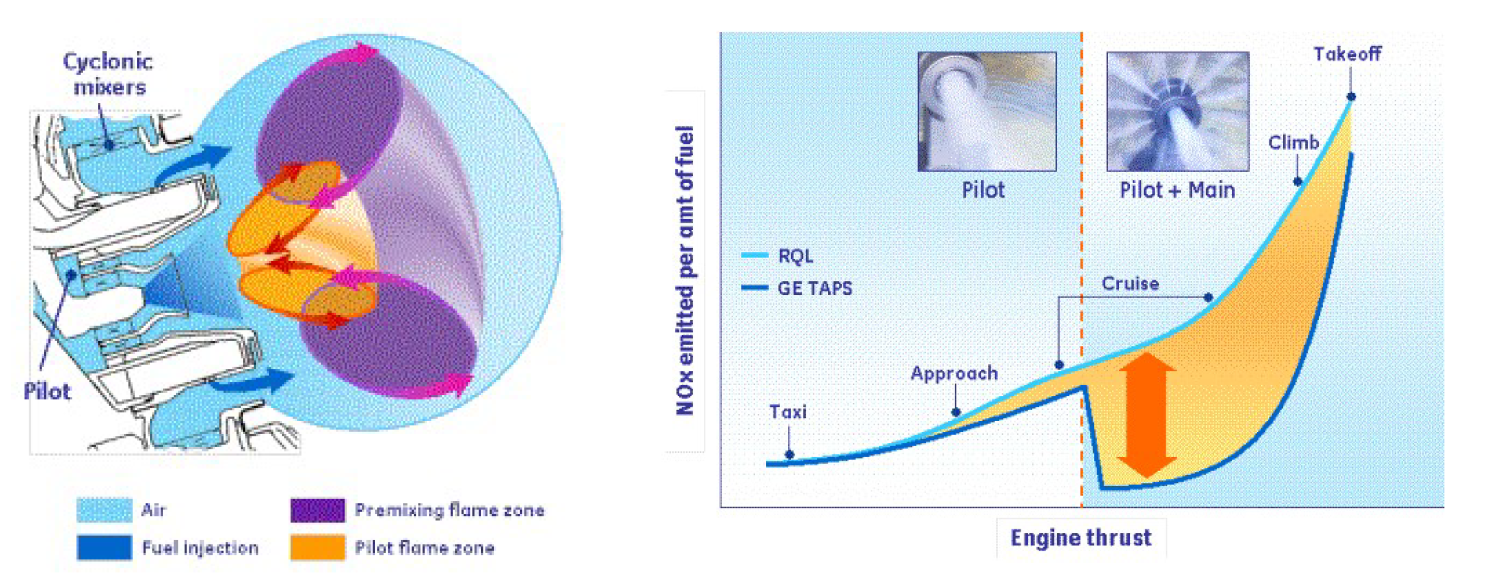
\includegraphics[scale=0.6]{./part0_intro/foust_TAPS}
	\caption{\textsl{Left}: regions in a multi-staged injection system from a TAPS concept. \textsl{Right}: effect of multi-staged injection in NO$_\mathrm{x}$ emissions from a TAPS concept compared to a RQL system. Source: \citeColor[foust_development_2012].}
	\label{fig:foust_TAPS}
\end{figure}

MSFI are a promising technology for fuel injection in aeronautical combustors, and manufacturers such as Safran are working in developing these systems for their application in future engines. Since their main characteristic is fuel staging, processes prior to combustion (such as injection, atomization and mixing) are fundamental for MSFI performance, and their proper comprehension is paramount to optimize such systems. The next sections makes a review on the two-phase flow physical mechanisms of injection and atomization relevant to these injection systems.


\section{Fuel injection technology}
\label{sec:ch1_fuel_injection_technology}

An example of a multipoint injector is shown in Figure \ref{fig:multipoint_injector_snecma}. Fuel is injected through two inlets: a central nozzle (the pilot stage), where fuel is injected with a pressure-swirl atomizer spreading as a \textbf{hollow cone} spray, and the multipoint injectors located in a crown around the central injector (the take-off stage), where fuel is injected in a \textbf{jet in crossflow} configuration. As seen in the figure, these two injection systems will produce atomization of the fuel shortly after the injection location. Furthermore, a third atomization mechanisms is if the opening angle of the hollow cone is large enough; in this case, liquid can impinge the walls of the injector and break due to the interaction with the aerodynamics and the liquid wall, forming an \textbf{airblast} spray. As a consequence of these three atomization mechanisms, a dispersed spray will be formed further downstream the injection chamber. This spray will be later able to evaporate, mix with the surrounding air and burn in the combustion process.

%\begin{figure}[ht]
%     \centering
%     \begin{subfigure}[b]{0.45\textwidth}
%         \centering
%         \includeinkscape[inkscapelatex=false,scale=0.35]{./part0_intro/multipoint_injector_snecma}
%     \end{subfigure}
%     %\hfill
%     \begin{subfigure}[b]{0.45\textwidth}
%         \centering
%          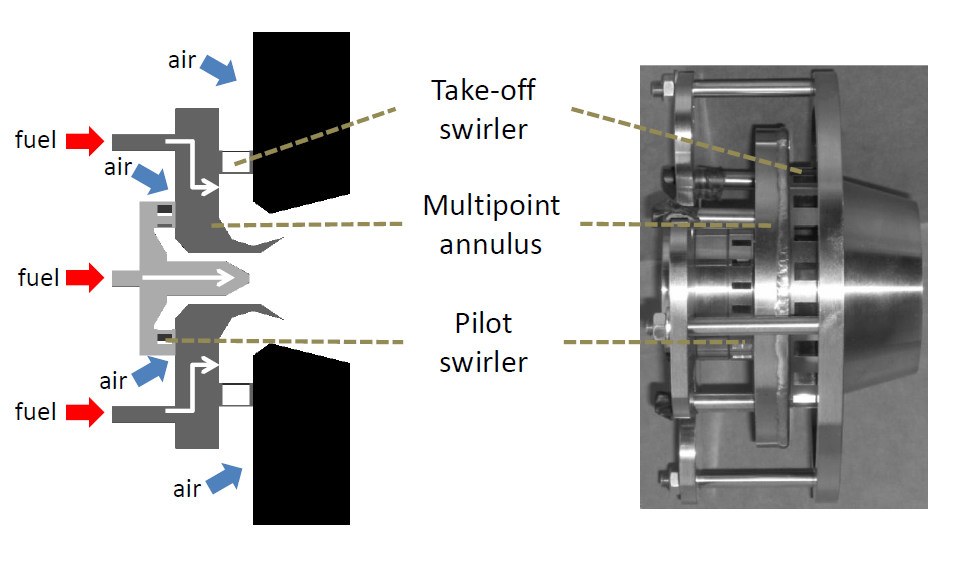
\includegraphics[scale=0.5]{./part0_intro/BIMER_swirler}
%     \end{subfigure}
%        \caption{\textsl{Left}: Size histogram evolution with accumulation time of droplets. \textsl{Right}: comparison of two droplet size histograms from two consecutive time instants.}
%	% See: https://stackoverflow.com/questions/35210337/can-i-plot-several-histograms-in-3d/35225919
%        \label{fig:multipoint_injectors}
%\end{figure}

\begin{figure}[ht]
     \centering
     \includeinkscape[inkscapelatex=false,scale=0.5]{./part0_intro/multipoint_injector_snecma}
      \caption{Multipoint injector from SNECMA (source: \citeColor[jaegle_large_2009]) showing the atomization mechanisms present in MSFI systems.}
      \label{fig:multipoint_injector_snecma}
\end{figure}

This thesis aims at studying the non-reactive processes of injection and atomization, but not the reactive phenomena of evaporation, mixing and combustion. Hence, in the subsequent sections the process of atomization is described. In particular, emphasis is done in the jet in crossflow configuration found in MSFI, which has been the object of study of this thesis.

\subsection*{The atomization process}

Liquid fuel injected into combustion chamber cannot be evaporated straightforward because the specific surface of fuel (i.e. the surface of fuel which is in contact with the continuous gas) is not high enough. Hence, this specific surface is increased by breaking the continuous liquid jet into smaller fragments in the process of atomization. \citepColor[lefebvre_atomization_2017] defines atomization as \textsl{the process by which a liquid jet or sheet is disintegrated by the kinetic energy of the liquid, by the exposure to
high-velocity air or gas, or by mechanical energy applied externally through a rotating or vibrating device}.

Atomization is triggered by instabilities which are found naturally in liquids jets. \citeColor[rayleigh_instability_1878] found that jet breakup oin smaller drops is produced due to the growth of small disturbances in the liquid. This disturbances are amplified by the aerodynamic interaction with the surrounding air, enhancing the energy transfer between both phases. Turbulence of the liquid jet also amplifies these disturbances: if the fuel is being injected in a turbulent state (i.e. at a high Reynolds number), atomization will occur promptly. 

Atomization is generally divided by the scientific community in two parts primary atomization and the secondary atomization. In primary atomization, the continuous liquid phase breaks into big ligaments and droplets. These fragments then split into small droplets during the secondary atomization. Figure \ref{fig:atomization_regimes_herrmann} shows a schematic sketch of liquid jet injection and the atomization process. Two main regimes of atomization are distinguished:

\begin{itemize}

	\item \textbf{Primary atomization}.  See the regimes in Figure \ref{fig:regimes_atomization_primary}.
	
	\item \textbf{Secondary atomization}.  See the regimes in Figure \ref{fig:regimes_atomization_secondary}.

\end{itemize}

\begin{figure}[h!]
	\centering
	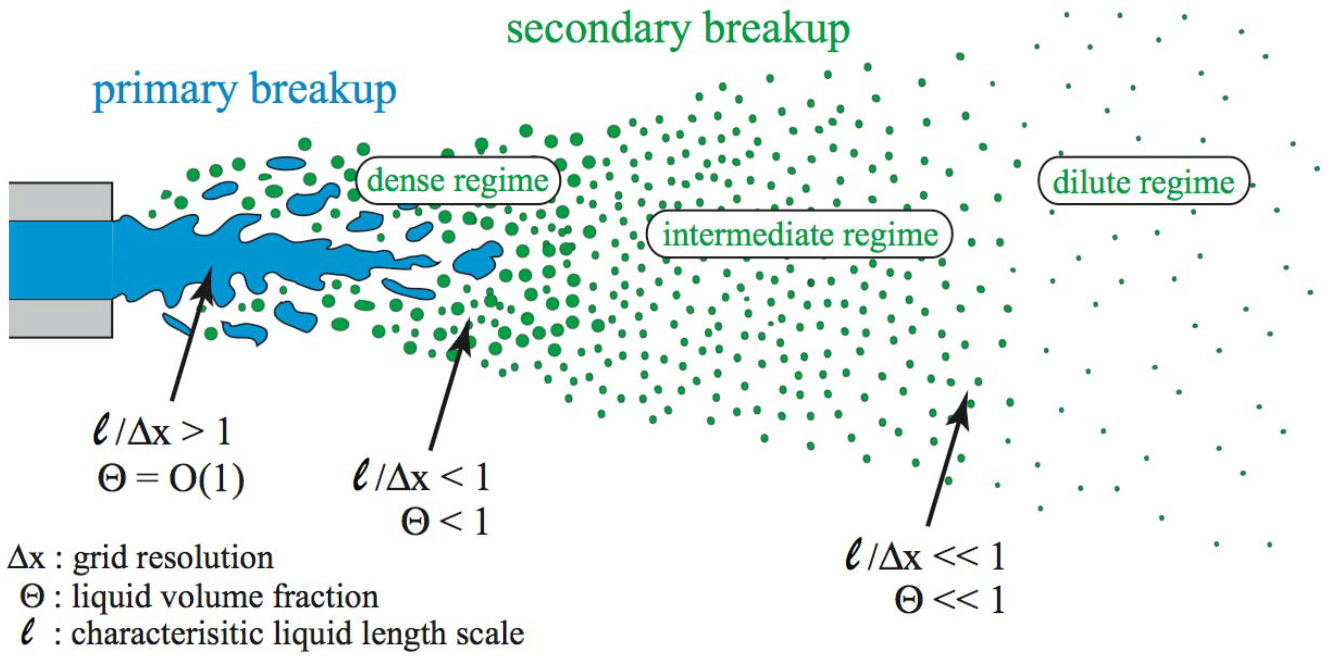
\includegraphics[scale=0.5]{./part0_intro/atomization-regimes-scheme}
	\caption{Atomization breakup regimes. Source: \citeColor[herrmann_modeling_2003]}
	\label{fig:atomization_regimes_herrmann}
\end{figure}

Explain two-phase flows phenomenology (injection + atomization) here. 

Explain airblast, hollow-cone, jicf.

\begin{figure}[h!]
	\centering
	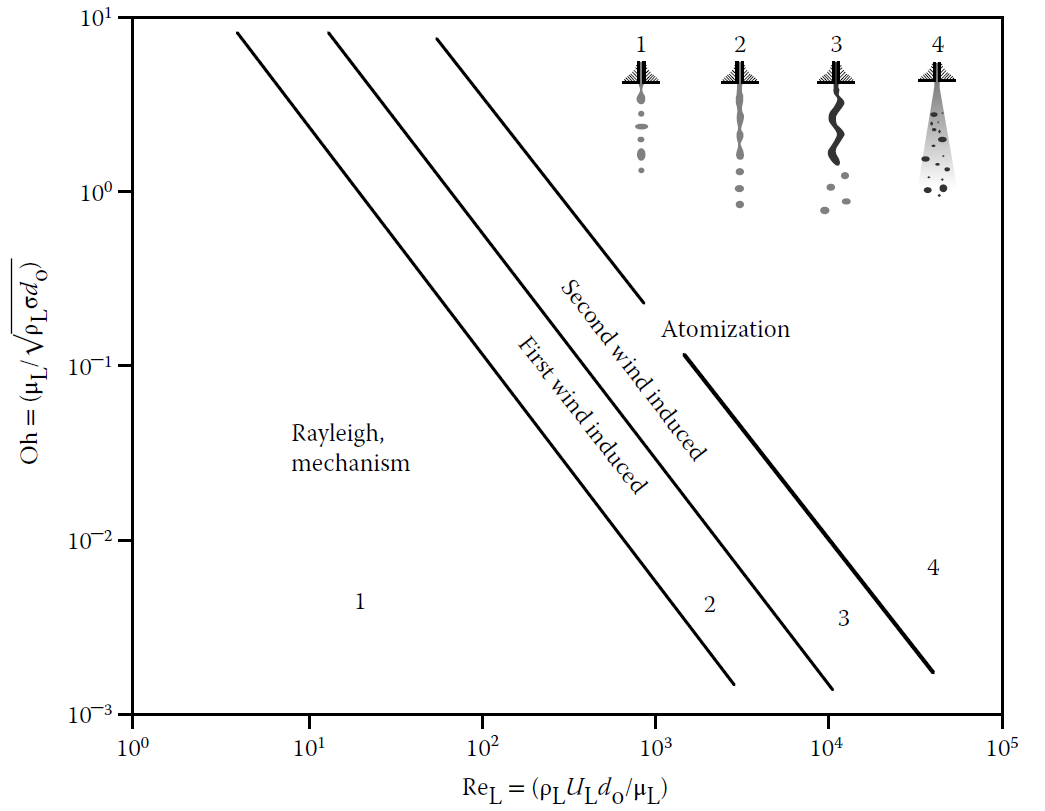
\includegraphics[scale=0.5]{./part0_intro/regimes_atomization_primary}
	\caption{Primary atomization regimes. Source: \citeColor[lefebvre_atomization_2017]}
	\label{fig:regimes_atomization_primary}
\end{figure}

\begin{figure}[h!]
	\centering
	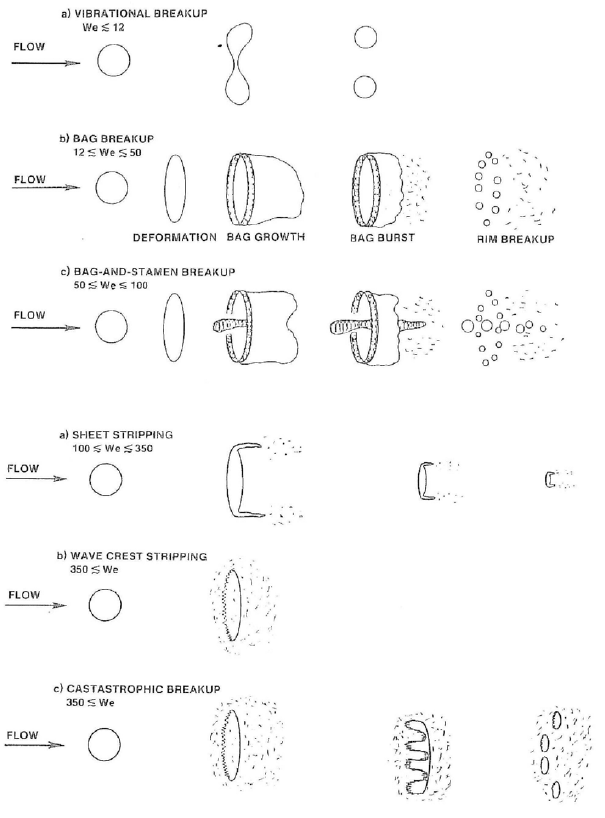
\includegraphics[scale=0.5]{./part0_intro/regimes_atomization_secondary}
	\caption{Secondary atomization regimes. Source: \citeColor[pilch_use_1987]}
	\label{fig:regimes_atomization_secondary}
\end{figure}


\subsection*{Jet in crossflow atomization}

In a liquid JICF, the liquid jet faces a transverse stream of air at the nozzle exit. The liquid jet is bended towards the trajectory of the airflow, and then starts to suffer from atomization. The aerodynamic interaction with the airflow and the inertia of the jet will be responsible for all the processes involved: it will influence
the penetration of the liquid jet, how fine and prompt the atomization will be and the later mixing with the air. In a reactive configuration, atomization will be followed by evaporation into gaseous fuel, mixing with air and finally combustion. Figure \ref{fig:JICF_multiphysics} illustrates all the multi-physical processes involved in a liquid JICF from fuel injection until combustion, relevant for the application inside future aeronautical combustors.


\begin{figure}[ht]
     \centering
     \includeinkscape[scale=0.75]{./part0_intro/JICF_multiphysics}
      \caption{Multi-physics phenomena in a reactive jet in crossflow. }
      \label{fig:JICF_multiphysics}
\end{figure}

The atomization process in liquid JICF has been studied experimentally by several authors \citemColor[adelberg_breakup_1968,wu_breakup_1997,becker_breakup_2002,freitag_spray_2008]. Their studies have identified two main mechanisms of primary breakup:

\begin{itemize}

	\item \textbf{Column breakup}. Surface waves on the liquid column start to grow until the jet breaks into ligaments,
which eventually turn into droplets during secondary atomization. An example is shown in Figure \ref{fig:JICF_breakup_mechanisms_freitag}
left, showing the surface waves caused by Kelvin-Helmholtz instabilities. This type of breakup occurs
when the aerodynamic interaction is not too strong (low relative liquid-air velocities).

\item \textbf{Surface breakup}. A strong aerodynamic interaction (large relative liquid-air velocity, high viscosity,
etc.) produces the disintegration of the liquid jet by means of shear. Ligaments and droplets are
stripped off the sides of the jet, which eventually is torn apart into droplets. Surface breakup can be
appreciated in Figure \ref{fig:JICF_breakup_mechanisms_freitag} right.

\end{itemize}


\begin{figure}[h!]
	\centering
	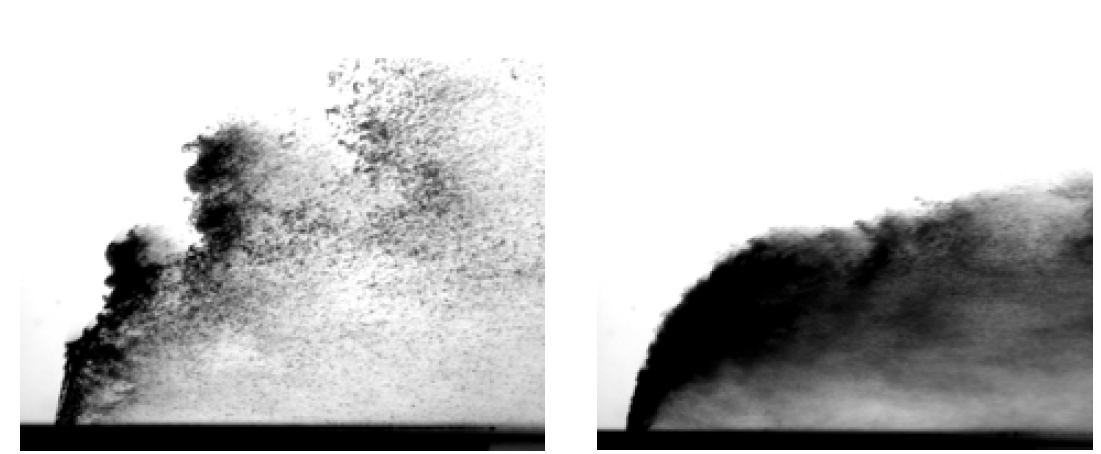
\includegraphics[scale=0.5]{./part0_intro/JICF_breakup-mechanisms_freitag}
	\caption{Experimental images of kerosene JICF breakup. \textsl{Left}: column breakup. \textsl{Left}: surface breakup. Source: \citeColor[freitag_spray_2008]}
	\label{fig:JICF_breakup_mechanisms_freitag}
\end{figure}

Explain trajectory, breakup/breakdown points, influences of parameters, breakup regimes.



\section{Objective and thesis outline}
    %\addcontentsline{toc}{section}{\protect\numberline{}Manuscript organisation}
    
The purpose of this thesis is to develop a new methodology to build lagrangian injectors for performing dispersed phase simulations. 

The thesis is divided in three main sections as follows:

\begin{itemize}

	\item \textbf{Part I} shows the state of the art in numerical methods to simulate two-phase flows. Different strategies are used depending on the atomization regimes as shown in Figure \ref{fig:atomization_regimes_herrmann}. Chapter \ref{ch2:numerical_methods_resolved_atomization} reviews methodologies aiming at resolving atomization, applicable to dense regimes and useful when the atomization dynamics need to be known, but out of scope for reactive simulations including combustion. Chapter \ref{ch3:disperse_phase_methods} discusses methodologies to simulate dispersed-phase problems, with a particular emphasis on the state of the art in lagrangian methodologies to simulate injection in MSI.
	
	\item \textbf{Part II} describes the design and application of the methodology developed in this thesis. This methodology is thoroughly described in Chapter . Then, application of this methodology to build lagrangian injectors in an academic non-reactive kerosene jet in crossflow test case is done in Chapter \ref{ch5:jicf_resolved_simulations}. The obtained injectors are then applied in the same configuration to initialise dispersed phase simulations in Chapter \ref{ch4:sli_development}.
	
	\item \textbf{Part III} focuses on the application of the injection models in an academic MSFI tested at EM2C named BIMER. An introduction to the test bench and simulations of the aerodynamic field are presented in Chapter \ref{ch9:bimer_test_bench_and_aero}. Then, Chapter \ref{ch8:bimer_resolved_atomization} describes resolved simulations of the atomization process in BIMER performed for one multipoint injector, from which lagrangian injectors are learnt. Finally, Chapter \ref{ch9:BIMER_lagrangian} shows the application of the learnt injectors to initialise lagrangian injection in the take-off stage of BIMER.

\end{itemize}

